\chapter{Zagadnienia teoretyczne}


\section{Sieci neuronowe}

Sieci neuronowe stanowią jedną z najpopularniejszych technik uczenia maszynowego. Są one inspirowane działaniem ludzkiego mózgu. Sieci składają się z neuronowów, pogrupowanych w połączone ze sobą warstwy.

Ogólna architektura sieci neuronowej:
\begin{itemize}
    \item Warstwa wejściowa - ta warstwa przyjmuje dane początkowe w formie tensora liczb rzeczywistych. Danymi wejściowymi mogą być poziomy jasności obrazu, dane o cenach lub sygnale (w przypadku prognozowania serii czasowych) lub osadzenia (z ang \textit{embeddings}) dla modeli językowych.
    \item Warstwy ukryte - te warstwy przetwarzają dane wejściowe przez sekwencję transformacji matematyczncyh. Neurony są połączone z poprzednią warstwą, a siła ich połączenia jest wyrażana przez tak zwane wagi. Wartość, którą przyjmie dany neuron jest liczona na podstawie ważonej sumy wartości neuronów z poprzedniej warstw. Po obliczeniu sumy, stosowana jest funkcja aktywacji. Ma ona za zadanie wprowadzić nieliniowość obliczeń, która jest wymagana do rozpoznawania zaawansowanych wzorców.
    \item Warstwa wyjściowa - warstwa, która generuje końcowy tensor. Tensor może zawierać informacje takie jak rozkład prawdopodobieństwa przyporządkowania do poszczególnych klas. Może również zawierać prognozowaną liczbę, w przypadku modeli regresyjnych.
\end{itemize}

Proces trenowania sieci neuronowej polega na modyfikowaniu wag pomiędzy połączeniami poszczególnych neuronów tak, by minimalizować różnicę między tensorem wyjściowym, a tensorem oczekiwanym.
Najczęściej stosuje się do tego zadania algorytmy optymalizacyjne oparte na pochodnych i gradientach. Przykładem może być \textit{algorytm spadku wzdłuż gradientu}.
W rzeczywistych zadaniach stosuje się jednak bardziej wyszukane algorytmy takie jak algorytm stochastycznego spadku wzdłuż gradientu albo algorytm \textit{Adam}.

Sieci neuronowe okazały się dużym sukcesem w wielu trudnych zadaniach uczenia maszynowego.
Są z powodzeniem stosowane w takich branżach jak medycyna, rozrywka, cyberbezpieczeństwo czy motoryzacja. Na przykład zespół Tesla Vision trenuje duże sieci neuronowe by stworzyć pojazd autonomiczny, zdolny poruszać się bezpiecznie bez kierowcy.
Sieci neuronowe coraz częściej będą wykonywać określone zadania szybciej i skuteczniej niż człowiek.
Czas reakcji systemu autopilot samochodu autonomicznego jest znacznie krótszy niż czas reakcji kierowcy, co w długiej perspektywie może przyczynić się do zwiększenia bezpieczeństwa na drogach i szlakach komunikacyjnych.
Innym bardzo ważnym zastosowaniem sieci neuronowych jest medycyna. Naukowcy z Google DeepMind stworzyli model \textit{AlphaFold}, który jest w stanie przewidywać molekularną strukturę białek.
Postęp informatyki w naukach biologicznych i chemicznych otwiera perspektywę na leczenie chorób, które dotychczas były nieuleczalne i umożliwia lepsze zrozumienie organizmu człowieka.


\section{Algorytm propagacji wstecznej}

Algorytm propagacji wstecznej to podstawowy algorytm używany do trenowania sieci neuronowych \cite{geron}.
Trenowanie sieci neuronowej to nic innego jak aktualizacja wag neuronów w taki sposób, by minimalizować tak zwany błąd (z ang. \textit{loss}) w predykcjach.

Zasada działania algorytmu:
\begin{itemize}
    \item Inicjalizacja - wagi neuronów są ustawiane na losowe wartości. Często wartości są losowane z rozkładu prawdopodobieństwa Glorota.
    Użycie takiego rozkładu pozwala uodpornić proces treningu na problem zanikających i eksplodujących gradientów.
    \item Przejście w przód - dane wejściowe są przekazywane do sieci neuronowej i liczone są wartości neuronów w kolejnych warstwach.
    Ostatnia warstwa stanowi wyjście modelu.
    \item Obliczenie błędu (inaczej straty) - wyliczone wyjście modelu jest porównywanie z oczekiwanym wyjściem (pochodzi ono z danych wejściowych w przypadku uczenia nadzorowanego).
    Używając różnych funkcji matematycznych, algorytm oblicza błąd, który informuje, jak bardzo predykcje odbiegają od docelowego wyjścia modelu.
    Najpopularniejsze funkcje błędu to błąd średniokwadratowy (z ang. \textit{Mean-Square Error} albo \textit{MSE}) bądź entropia krzyżowa (z ang. \textit{Cross Entropy}).
    Dla zadań klasyfikacji wieloklasowej często stosuje się entropię krzyżową, zaś dla regresji liniowej (np.
    przewidywanie ceny nieruchomości) można zastosować błąd średniokwadratowy.

    Błąd średniokwadratowy dany jest wzorem \ref{eq:mse}, gdzie $n$ to liczba obserwacji, $y_i$ to rzeczywista wartość dla $i$-tej obserwacji $\hat{y}_i$ to przewidywana wartość dla $i$-tej obserwacji.
    \begin{equation}
        \text{MSE} = \frac{1}{n} \sum_{i=1}^{n} (y_i - \hat{y}_i)^2\label{eq:mse}
    \end{equation}

    Z kolei funkcja błędu entropii krzyżowej dana jest wzorem \ref{eq:cross_entropy}, gdzie $N$ to liczba wszystkich próbek, a $K$ to liczba klas. $y_{i,k}$ to prawdziwa etykieta dla próbki $i$ i klasy $k$, a $\hat{y}_{i,k}$ to przewidywane prawdopodobieństwo, że próbka $i$ należy do klasy $k$.
    \begin{equation}
        \mathcal{L}_{CE} = -\frac{1}{N} \sum_{i=1}^{N} \sum_{k=1}^{K} y_{i,k} \log(\hat{y}_{i,k})\label{eq:cross_entropy}
    \end{equation}

    \item Propagacja błędu - błąd jest przekazywany wstecz od warstwy wyjściowej, przez warstwy ukryte aż do warstwy wejściowej.
    Przy przekazywaniu, liczone są pochodne cząstkowe funkcji błędu względem każdej z wag.
    \item Aktualizacja wag - wagi neuronów są aktualizowane za pomocą różnych algorytmów optymalizacyjnych.
    Jednym z najprostszych algorytmów jest metoda najszybszego spadku wzdłuż gradientu, która sprowadza się wyliczenia następnej wartości za pomocą równania \ref{eq:fastest_gradient_descent}.
    Warto zwrócić uwagę na hiperparametr $\alpha_k$ - jest to współczynnik uczenia.
    Informuje on algorytm o tempie optymalizacji.
    Gdy współczynnik będzie zbyt niski, proces trenowania będzie trwał bardzo długo i może dojść do sytuacji, gdzie model nigdy nie zdąży się wytrenować.
    Z kolei zbyt wysoka wartość współczynnika uczenia może spodować trudności ze znalezieniem minimum globalnego i brak poprawy jakości modelu.
    \begin{equation}
        x_{k+1} = x_k - \alpha_k \nabla f(x_k)\label{eq:fastest_gradient_descent}
    \end{equation}
    \item Iteracja - kroki (oprócz inicjalizacji) są powtarzane tak długo, aż sieć neuronowa będzie dawała jakościowe predykcje.
\end{itemize}

Zagadnienie propagacji wstecznej jest bardzo szerokie - pomimo niezbyt skomplikowanego algorytmu, w trakcie trenowanie sieci mogą pojawiać się problemy z tak zwanymi zanikającymi bądź eksplodującymi gradientami.
Wartość współczynnika uczenia nie musi być z góry ustalona, lecz może być wyliczana na bieżąco.
Przykładowo, wraz z czasem treningu współczynnik może być zmniejszany (nazwa metody w j. ang. to \textit{learning rate decay}).
Podsumowując, propagacja wsteczna jest bardzo przydatna w zagadnieniu trenowania sieci neuronowych i uczeniu głębokim, pomimo korzystania z prostych pojęć analizy matematycznej takich jak pochodna cząstkowa.


\section{Splotowe sieci neuronowe}

Splotowe sieci neuronowe to rodzaj sieci neuronowych dedykowany do rozpoznawania przede wszystkim cech obrazów \cite{geron}.
Znajdują one zastosowanie w zadaniach takich jak klasyfikacja obrazów, rozpoznawanie obiektów lub segmentacja.
Czasem są one używane do analizy wideo lub analizy sygnału w czasie.

Struktura splotowych sieci neuronowych sprowadza się do:
\begin{itemize}
    \item Warstwa wejściowa - ta warstwa przyjmuje zazwyczaj obraz jako tensor jasności poszczególnych pikseli.
    Obraz wejściowy może być w skali szarości (pojedynczy kanał) lub kolorowy - najczęściej składowe RGB pojedynczego piksela są kodowane przez 3 neurony.
    \item Warstwy splotowe - te warstwy wykorzystują matematyczną operację splotu.
    Taka warstwa zawiera pewną macierz, zwaną filtrem o pewnym ustalonym rozmiarze (najczęściej \textit{3x3} lub \textit{5x5}).
    Macierz ta jes przesuwana od lewej do prawej, z góry do dołu po obrazie.
    Odpowiednie wartości filtra są w stanie wzmocnić lub osłabić pewne cechy obrazu takie jak ostre krawędzie bądź rogi.
    Wartości macierzy są dobierane w procesie trenowania modelu.
    \item Warstwy łączące - warstwy te mają za zadanie zmniejszyć wymiarowość danych z poprzedniej warstwy.
    Popularną funkcją łączącą jest uśrednianie - dla zadanego otoczenia pikseli (najczęściej \textit{2x2} lub \textit{3x3}) wybierana jest średnia wartość.
    Inną funkcją łączącą jest maksimum - z otoczenia wybierana jest wartość maksymalna.
    \item Warstwy gęste - po kilku warstwach splotowych, zaawansowane rozumowanie jest przeprowadzane przez warstwy gęste, czyli neurony połączone w sposób "każdy z każdym".
\end{itemize}

Główne zastosowanie splotowych sieci neuronowych to wykrywanie przedmiotów i ludzi na obrazach i nagraniach wideo,
opisywanie i wykrywanie anomalii w skanach medycznych oraz analiza sytuacji na drodze dla pojazdów autonomicznych.


\section{Problem klasyfikacji komórek krwi w rozmazach szpiku kostnego}

Problem opisu komórek na rozmazach krwi i szpiku kostnego jest bardzo ważny z perspektywy diagnostyki wielu chorób takich jak np.
nowotwory.
Po wykonaniu mikroskopowej fotografii rozmazu lekarz diagnosta musi policzyć ilość każdego typu komórek w próbce.
Ilość komórek danego rodzaju może być przesłanką do zdiagnozowania nieprawidłowości w organiźmie.
Przykładowo, do stwierdzenia białaczki lekarz zlicza ilość limfoblastów w próbce w stosunku do wszystkich komórek.
Gdy ten stosunek przekracza pewien próg, jest to przesłanka o obecności nowotworu.
Limfoblasty to forma niedojrzała limfocytów.
Ich zwiększone występowanie sugeruje nieprawidłowości w procesie rozwoju tych komórek do docelowej postaci.

Rodzaj komórki można stwierdzić przede wszystkim na podstawie jej wyglądu po barwieniu.
Zwraca się uwagę na wielkość jądra w stosunku do cytoplazmy, występowanie jąderek oraz ziarnistości \cite{histology}.

Elementy morfotyczne krwi przedstawia rys. \ref{fig:electron_microscope}.
Górna część rysunku przedstawia obraz z mikroskopu optycznego, zaś dolna - z mikroskopu elektronowego, gdzie widoczne jest więcej szczegółów.
Objaśnienie: A - erytrocyt (widok z góry i widok przekroju), B - neutrofil, C - eozynofil, D - bazofil, E - limfocyt, F - monocyt. “za“ - ziarna azurochłonne, “zs“
- ziarna swoiste.

\begin{figure}
    \centering
    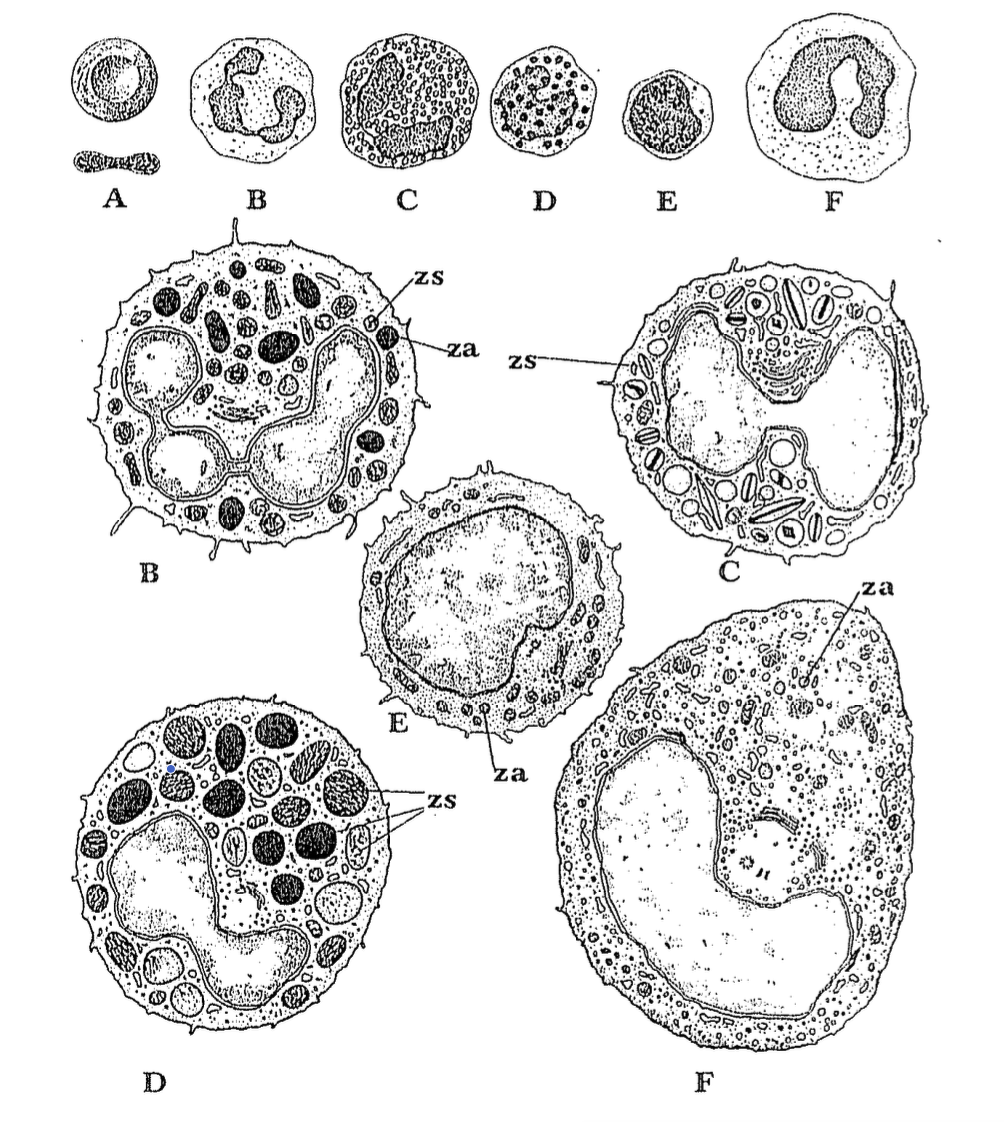
\includegraphics[width=0.8\textwidth]{morfotyczne}
    \caption{Elementy morfotyczne krwi w obrazie optycznego i elektronowego. Rysunek pochodzi z “Kompendium histologii“ autorstwa Tadeusza Cichockiego, Jana Litwina i Jadwigi Mireckiej \cite{histology}.}
    \label{fig:electron_microscope}
\end{figure}

Rozwój metod komputerowej klasyfikacji komórek jest bardzo istotny, ponieważ potencjalne zautomatyzowanie procesu zliczania komórek pozwoliłoby szybsze stawianie diagnozy i zaoszczędzenie wielu godzin pracy diagnostów.
%TODO check if this is truth
Obecne rozwiązania służące do opisu komórek w krwi lub szpiku kostnym bazują cytometrii przepływowej (czyli analizie kąta odbicia fali światła).
Warto natomiast zwrócić uwagę na to, że zdjęcie komórki (to znaczy obrazowanie w zakresie światła widzialnego) jest wystarczające do rozpoznania typu komórki przez człowieka, a więc niesie dostateczną ilość informacji.
To oznacza, że odpowiednio zaawansowany model sztucznej inteligencji byłby w stanie klasyfikować komórki jedynie na podstawie wizji komputerowej, bez potrzeby analizy widma falowego lub kątów odbicia światła.


\section{Algorytmy widzenia komputerowego}

W niniejszym projekcie, oprócz widzenia komputerowego realizowanego przez splotowe sieci neuronowe, wykorzystano również inne algorytmy do analizy obrazów.
Jednym z nich jest mechanizm \textbf{progowania obrazu} (z ang. \textit{thresholding}).
Operacja ta przyporządkowuje wartość maksymalną piksela na obrazie wyjściowym, gdy poziom jasności na obrazie wejściowym jest większy od zadanego progu $k$.
Analogicznie, wyjściowy piksel przyjmuje wartość minimalną (najczęściej $0$), gdy piksel wejściowy jest poniżej progu $k$ lub wartość jest równa (zob. równanie \ref{eq:thresholding}).

\begin{equation}
    T(x, y) =
\begin{cases}
0 & \text{jeśli } I(x, y) < k \\
1 & \text{jeśli } I(x, y) \geq k
\end{cases}\label{eq:thresholding}
\end{equation}

Inną ważną metodą widzenia komputerowego są \textbf{momenty Hu} (zwane też momentami obrazów).
Momenty Hu to zestaw metryk służących do opis kształtu i właściwości pewnego regionu obrazu \cite{vision}.
Korzystają one z analizy rozkładu jasności pikseli w obrazie.
W algorytmie ekstrakcji obrazów komórek z dużego zdjęcia rozmazu wykorzystywane są momenty centralne do wyznaczania punktów centralnych komórek.
Wzór na tak zwany moment centralny $\mu_{ij}$ przedstawia równanie \ref{eq:central_moment}, zaś współrzędne punktu centralnego można wyznaczyć korzystając z równań \ref{eq:centroid}.

\begin{equation}
    \mu_{ij} = \sum_x \sum_y x^i y^j I(x, y)\label{eq:central_moment}
\end{equation}

\begin{equation}
    \bar{x} = \frac{M_{10}}{M_{00}}, \quad \bar{y} = \frac{M_{01}}{M_{00}}\label{eq:centroid}
\end{equation}


\section{GradCAM - wytłumaczalne uczenie maszynowe}